%%%%%%%%%%%% INTRODUCCIÓN  %%%%%%%%%%%%

\begin{center}
	{\fboxrule=4pt \fbox{\fboxrule=1pt
		\fbox{\LARGE{\bfseries Introducción}}}} \\
	\addcontentsline{toc}{chapter}{Introducción}
	\rule{15cm}{0pt} \\
\end{center}

\pagenumbering{roman}
 
 \lettrine[lines=3, depth = 0]{E}{n} este documento explicar\'e c\'omo he llevado a cabo el proyecto final de prácticas para la asignatura \textbf{Arquitectura de Redes} que consiste en realizar la configuraci\'on de las redes de dos organizaciones diferentes (organizaci\'on A y B) siguiendo las especificaciones indicadas en el gui\'on del proyecto.
 
\par Para la simulación de estas redes e implementación del proyecto utilizaré el programa \textbf{Packet Tracer} de Cisco. Antes de ello he desarrollado sobre el papel el direccionamiento de las dos redes, tomando las decisiones que considero necesarias para optimizar el reparte de direcciones IP.
\par Lo siguiente que haré será configurar indipendientemente cada una de las redes de las dos organizaciones, de forma que cada una utilice un protocolo de encaminamiento diferente: 
 \begin{itemize}
 	\item \textbf{Organización A} $\rightarrow$ Protocolo RIP.
	\item \textbf{Organización B} $\rightarrow$ Protocolo OSPF.
 \end{itemize}
\par De esta forma permitiré la conmutación de paquetes dentro de la red de cada organización.
\par El objetivo final, mostrado en la figura \ref{fig:topologia} será interconectar las redes de ambas organizaciones para que pueda existir la conmutación entre ellas y obtener un esquema totalmente funcional al mismo tiempo que responderé a las preguntas que se plantean en cada uno de los apartados.

 %%% IMAGEN DE TOPOLOGÍA DE RED FINAL %%%
\begin{figure}[H]
	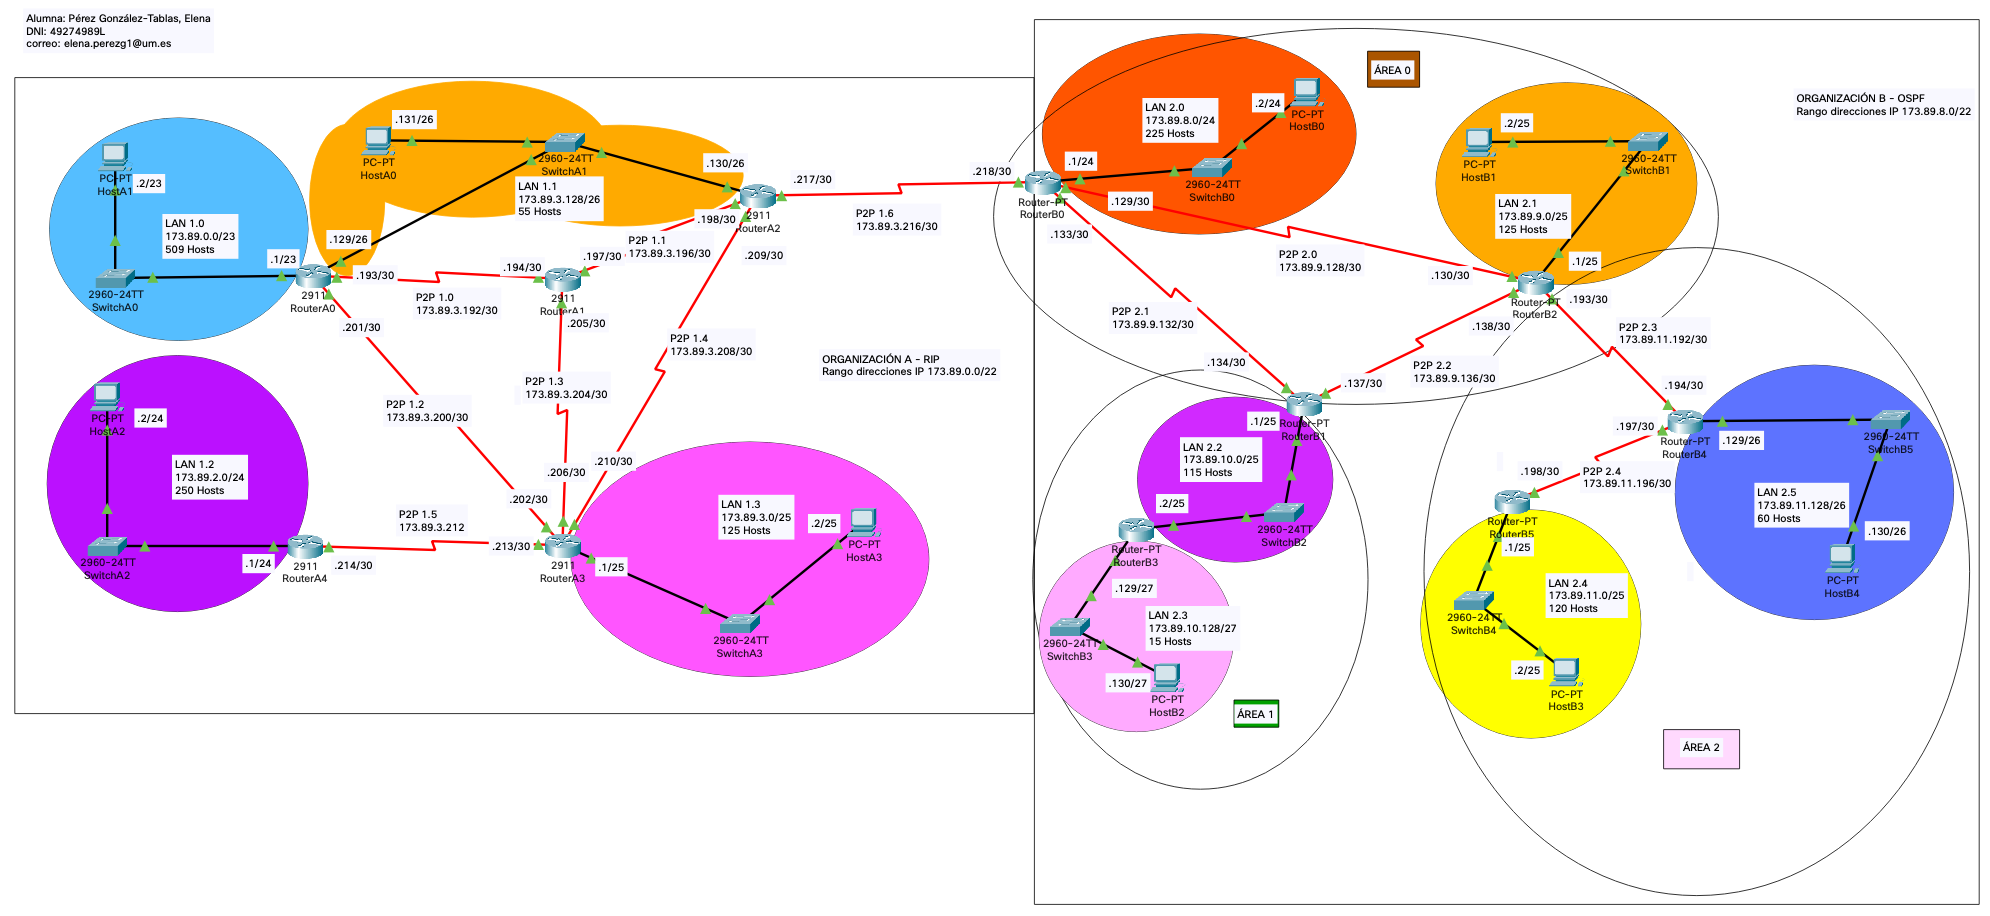
\includegraphics[width=\textwidth]{topologiaFinal}
	\centering
	\caption{Topología Final.}
    	\label{fig:topologia}
\end{figure}


\newpage
\pagenumbering{arabic}